\documentclass[11pt]{article}
\usepackage[utf8]{inputenc}	% Para caracteres en español
\usepackage{amsmath,amsthm,amsfonts,amssymb,amscd}
\usepackage{multirow,booktabs}
\usepackage[table]{xcolor}
\usepackage{fullpage}
\usepackage{lastpage}
\usepackage{enumitem}
\usepackage{fancyhdr}
\usepackage{mathrsfs}
\usepackage{wrapfig}
\usepackage{setspace}
\usepackage{calc}
\usepackage{multicol}
\usepackage{cancel}
\usepackage[retainorgcmds]{IEEEtrantools}
\usepackage[margin=3cm]{geometry}
\usepackage{amsmath}
\newlength{\tabcont}
\setlength{\parindent}{0.0in}
\setlength{\parskip}{0.05in}
\usepackage{empheq}
\usepackage{framed}
\usepackage[most]{tcolorbox}
\usepackage{xcolor}
\colorlet{shadecolor}{orange!15}
\parindent 0in
\parskip 12pt
\geometry{margin=1in, headsep=0.25in}
\theoremstyle{definition}
\newtheorem{defn}{Definition}
\newtheorem{reg}{Rule}
\newtheorem{exer}{Exercise}
\newtheorem{sln}{Solution}
\newtheorem{note}{Note}
\begin{document}
\setcounter{section}{0}
\title{Math lecs 15,16,17 review}

\thispagestyle{empty}
\begin{center}
{\LARGE \bf Lectures 15,16,17}\\[0.3cm]
{\large \bf Math301}\\[0.3cm]
Fall 2020
\end{center}
\tableofcontents
\newpage
\section{Homogeneous Linear ODEs of Second order} 
\subsection{What is an ODE ordinary differential equation?}
it's a mathematical model that relates some independent variable $X$ with a dependent variable $Y$ and it's derivatives.  
\begin{note}
the independent variable $x$ can either be in the equation or not. 
\end{note}
\subsection{What is the order of a linear ODE?}
it's the \textbf{highest order derivative} in the equation. 
\subsection{Linear ODEs of Second Order}
as we said before they are Linear ODEs with the highest order derivative is 2 and takes the following form: 
\begin{equation}
    F(x,y,y',y'')=0
\end{equation}
\subsection{Linear?}
A second order ODE can be called linear if the function $F$ in equation (1) is \textbf{Linear} in $y,y'$ and $y''$. So it can be put in the \textbf{Standard form}.
\begin{equation}
    y''+p(x)y'+q(x)y=r(x)
\end{equation}
the following ODE is \textbf{NOT Linear.}

\begin{equation}
    y''y+(y')^2=0
\end{equation}

\subsection{Homogenous Linear ODEs of Second Order}

same as we said before but $r(x)=0$ in the equation (2).
\begin{equation}
\label{H}
    y''+p(x)y'+q(x)y=0
\end{equation}

\subsection{What  is the solution of an ODE of Second order?}
the solution is a function $y=h(x)$ defined on $[a,b]$ ($I$) with some constraints: 
\begin{itemize}
    \item $h(x)$ is defined and twice differentiable on the interval $I$.
    \item Substituting with $h(x)$ and it's derivatives satisfies the equation.
    \begin{equation}
        F(x, h(x), h'(x), h''(x)) = 0
    \end{equation}
    
\end{itemize}

\subsection{IVPs initial value problems}

they are ODEs which have initial values.

\subsection{How to solve IVPs?}
nothing new! you just solve the ODE and afterwards you substitute with the values given as initial values so that you remove any constant $c$ in the solution $h(x)$ with it's original value. 
\begin{shaded}
\begin{equation} 
\begin{split} 
  y''+p(x)y'+q(x)y=r(x) \\
  y'(x_0) = k_1 \\
  y(x_0) = k_2\\
  \end{split} 
\end{equation}
\end{shaded}

The solution of an \textbf{IVP} is called a \textbf{particular solution}.
\subsection{Existence and Uniqueness Theorem for the Initial Value Problems}

If the coefficients $p(x), q(x)$ and $r(x)$ in ODE (2) are continuous
on an interval $I$ and if $x_0\in I$, the initial value problem (IVP) has a unique solution.

\subsection{Superposition Principle}
\begin{reg}if $y_1(x), y_2(x)$ are solutions of the linear homogenous ODE (4) then: any \textbf{linear comination} of  $y_1(x)$ and $y_2(x)$ is also a solution of the ODE.
\end{reg}
so the general soltion of an ODE which has two solutions is:
\begin{equation}
    y_G = c_1 y_1(x)+c_2 y_2(x) 
\end{equation}
\subsection{Linearly independent solutions}
two solutions are said to be linearly independent if $y_1$ and $y_2$ are not proportional on $I$, which means
\begin{equation}
    y_1(x) \neq ky_2(x) \text{where k is a constant}
\end{equation}
\begin{reg}
if neither $y_1$ nor $y_2$ is equal to 0 then they're linearly independent if : $\frac{y_1(x)}{y_2(x)} \neq  const.$
\end{reg}
\begin{exer}

Show that $y_1 = e^x$ and $y_2 = xe^x$ are two linearly independent solutions over $\Re$ of the ODE:
\begin{equation}
    y'' - 2y' + y = 0.
\end{equation}
\end{exer}
\begin{sln}
\begin{equation}
\begin{split}
    y''_1(x) -2y'_1(x) + y_1(x) = e^x -2e^x+e^x = 0\\
    y''_2(x) -2y'_2(x) + y_2(x) = xe^x+e^x+e^x - 2(xe^x+e^x) +xe^x = 0
    \end{split}
\end{equation}
and since $\frac{y_1}{y_2} = \frac{
1}{x} \neq const.$ Hence the two solytions are linearly independent solutions over $\Re$ .
\end{sln}
\begin{reg}
if the coeffecients p(x) and q(x) of the homogeneous equation 
\begin{equation}
    y''+p(x)y'+q(x)y=0
\end{equation}
are \textbf{continous} over the an interval $I$ then every slution has the following form 
\begin{equation}
    y = c_1 y_1(x)+c_2 y_2(x) 
\end{equation}
where $y_1(x)$ and $y_2(x)$ are any linearly independent solutions the ODE.
\end{reg}
\begin{note}
if two linearly independent solutions of (H)
have been found, then any other particular solution can be found from the general solution. Thus, solving the ODE boils down to finding two linearly independent solutions.
\end{note}
\subsection{Show that $y_1,y_2$ for a basis of the ODE}
\begin{enumerate}
    \item you differentiate and substitute in the ODE to prove it
    \item show that the solutions are linearly independent 
\end{enumerate}
\subsection{Reduction of Order Method of solving ODE}
this method means simply finding the general solution of a linear second order ODE using merely one solution.
\begin{enumerate}
    \item try to find the first solution of the ODE if not given (like assuming the solution is a power function and our goal is to find the power)
    \item using the superposition principle we assume that the other solution is $y_2 = u(x) y_1$ so our goal is to find u(x)
    \item differentiate $y_2$ twice and substitute.
    \item the reduction of order comes when you substitute and simplify you will remove $u''(x)$ and put $w'(x)$ instead.
    \item after finding $w$ a simple integration would get us $u$
\end{enumerate}
\begin{exer}
\begin{equation}
\label{E}
    (x^2 - x)y'' -  xy' + y = 0
\end{equation}
\begin{itemize}
    \item Show that the ODE (\ref{E}) has a solution $y_1$ that is a power function.
\item find a solution $y_2$ using reduction of order method.
\item deduce the general solution
\end{itemize}
\end{exer}
\begin{sln}
\begin{shaded}
First let $y_1 = x^p$ \\
\begin{equation}
\begin{split}
y_1' = px^{p-1}  \\
y_1'' = p (p-1) x^{p-2}\\
   (x^2-x)( p (p-1) x^{p-2}) -x * px^{p-1} + x^p =0\\
   (p-1) [(p-1)x^p-px^{p-1}]=0 \\ 
   &p=1 \\
   &y_1 = x\\
  &y_2 = x u(x) 
   \end{split}
\end{equation}
\end{shaded}
$y'_2 = u + xu'$ and $y''2 = 2u' + xu''$.
y2 is a solution of (\ref{E}) if it satisfies the equation. Substitution and simplification imply that
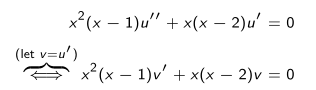
\includegraphics[scale =0.7]{images/sln2.png}\\
\begin{center}
    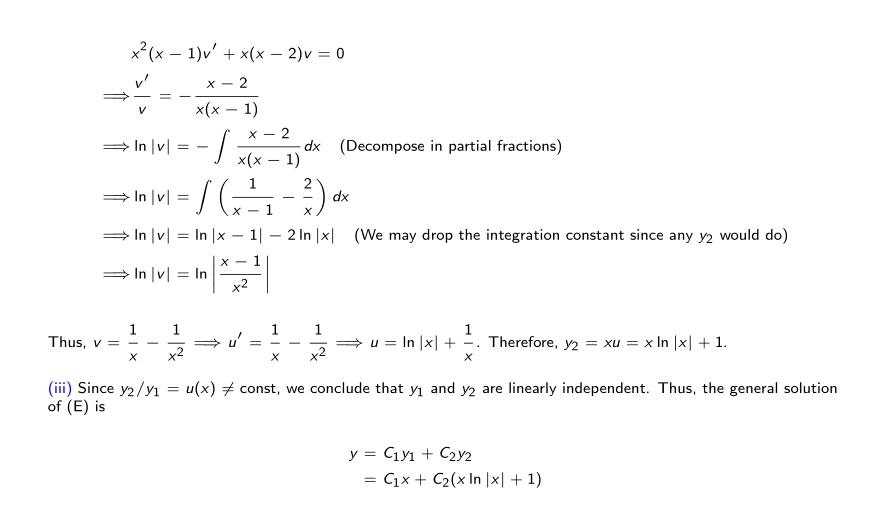
\includegraphics[scale=0.6]{images/sln1.png}
\end{center}
\end{sln}
\section{Homogeneous Linear ODEs with Constant Coefficients}
constant coeffecients means that $p(x)$ and $q(x)$ are constant in (\ref{H}) :) \\
and to solve this kind of ODE we use the following table :
\begin{center}
    \begin{tabular}{c|c}
       Roots of the \textbf{characteristic (or auxiliary)} equation   & General Solution \\
       \hline
        $\lambda_1, \lambda_2$ are \textbf{Real} and \textbf{Distinct}  & $y = C_1 e^{\lambda_1 x} + C_2 e^{\lambda_2 x}$\\
        \hline
        $\lambda_1, \lambda_2$ are \textbf{Equal}. $\lambda_1 = \lambda_2 =\lambda$ & $y = (C_1 + C_2 x) e^{\lambda x}$  \\
        \hline
        $\lambda_1, \lambda_2$ are \textbf{Complex}: $\alpha \pm \beta i$ & $y=e^{\alpha x} (C_1 cos(\beta x) + C_2 sin(\beta x))$
    \end{tabular}
\end{center}
The previous table can be easily deduced if you suppose that the solution of (H) is $y = e^{\lambda x}$ so we notice that $ y' = \lambda e^ \lambda x $ and $y'' = \lambda^2 e^ {\lambda x}$ so we see that the auxiliary equation can be extracted from the ODE as follows : 
\begin{align*}
    y'' + ay'+by &= 0 &
    \lambda^2 + a\lambda + b&=0 
    \end{align*}
    We can solve this system using the old known \textbf{polynomial} solution or using any other method like \textbf{Cramer's}. 
    \begin{align*}
    \omega &= \sqrt{a^2-4*b} &
    \lambda &= \frac{-a \pm \omega}{2}
    \end{align*}
 \section{Nonhomogeneous Linear ODEs with constant coefficients}
in order to solve this kind of linear ODEs we use the help of the following rule:
\begin{reg}
the general solution of a nonhomogeneous
ODE is the sum of the general solution of its complementary equation and any particular solution: $y_H = y_G - y_p$ \textbf{Hence} $y_G = y_H + y_p$.
\end{reg}
\subsection{Where did this information come from ?! }
Let's look at the following nonhomogeneous equation:
\begin{align*}
    y''+p(x)y'+q(x)y=r(x) && \text{ (NH)}
\end{align*}
If $y_G$ is the general solution of (NH) and $y_p$ is just any particular solution, then their difference $y_H = y_G - y_p$ is the general solution of the homogeneous equation
\begin{align*}
    y''+p(x)y'+q(x)y=0 && \text{ (H)}
\end{align*}
where a and b are the same as in (NH).The ODE (H) is called the complementary equation of (NH).
In fact,
\begin{center}
    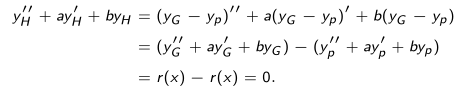
\includegraphics[]{images/eqn.png}
\end{center}
\subsection{Solving NH Linear ODEs}
Since we have a recipe for the general solution of the complementary equation (H), solving (NH) boils down to finding any particular solution yp.\\
We can do this using one of the following methods :
\begin{itemize}
    \item Method of undetermined coeffecients
    \item Method of variation of parameters
\end{itemize}

\subsection{Method of undetermined coeffecients}
from its name: we have some coeffiects that are undetermined/unknown yet and we want to find them. Look at the following table 
\begin{center}
    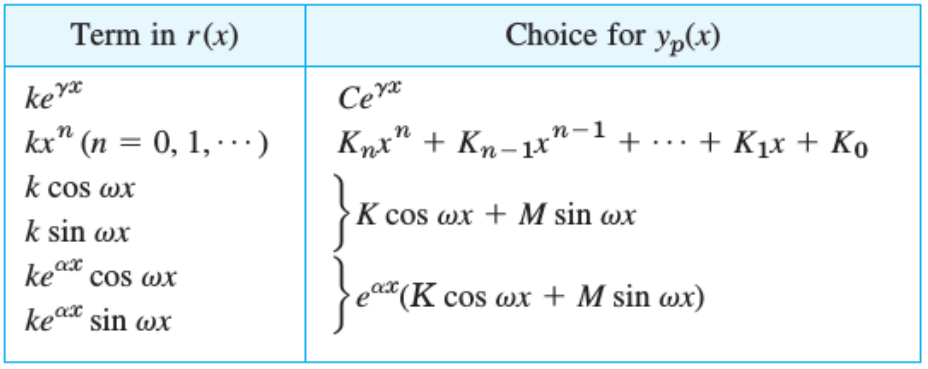
\includegraphics[scale=0.45]{images/undet.png}
\end{center}
So the method is simply as follows: 
\begin{enumerate}
    \item find $y_H$ using the complementry equation.
\item use the suggested $y_p(x)$ from the table
\item check linear independence 
\begin{enumerate}
    \item if the suggested $y_p$ is linearly independant with each term of $y_H$ you do nothing
    \item if not multiply $y_p$ by $x$ and check again
    \begin{enumerate}
        \item if LI do nothing
        \item else multiply by $x$
        \begin{enumerate}
            \item ...
        \end{enumerate}
    \end{enumerate}
\end{enumerate}
\item substitute in (NH) with $y_p$ to find the coeffecients.
\item deduce $y_G$
\end{enumerate}
\begin{reg}
\textbf{Modification rule}: is simply the 3rd step in the previous list, or you can follow this text: \\
If r(x) is one of the terms in the adjacent table but is actually a solution of the complementary equation $y'' + ay' + by = 0$, then \begin{enumerate}
    \item multiply the suggested yp by x in case $r(x)$ corresponds to a simple root of the complementary equation (H).
    \item multiply the suggested $y_p$ by $x^2$ in case $r(x)$ corresponds to a double root of the complementary equation (H).
\end{enumerate} 

\end{reg}
\begin{reg}
\textbf{Sum rule}
If $r(x)$ coressponds to the sum of two of the listed functions in the previous table then you can either \begin{enumerate}
    \item attempt $y_p$ as the sum of the two suggested solutions .
    \item attempt each $y_p$ alone and then $y_p = y_{p1} + y_{p2}$
\end{enumerate}
\end{reg}
\begin{reg}
\textbf{Product rule}
\begin{enumerate}
    \item If $r(x) = P(x) e^{mx}$ then attempt $y_p = Q(x) e^{mx}$  where $P$ and $Q$ are degree polynomials
    \item If $r(x) = P(x) e^{mx} cos(kx)$ or $r(x) = P(x) e^{mx} sin(kx)$ attempt $y_p = Q(x) e^{mx} cos(kx) + R(x) e^{mx} sin(kx)$
\end{enumerate}
\end{reg}
\subsection{Lecture Examples}
\begin{center}
    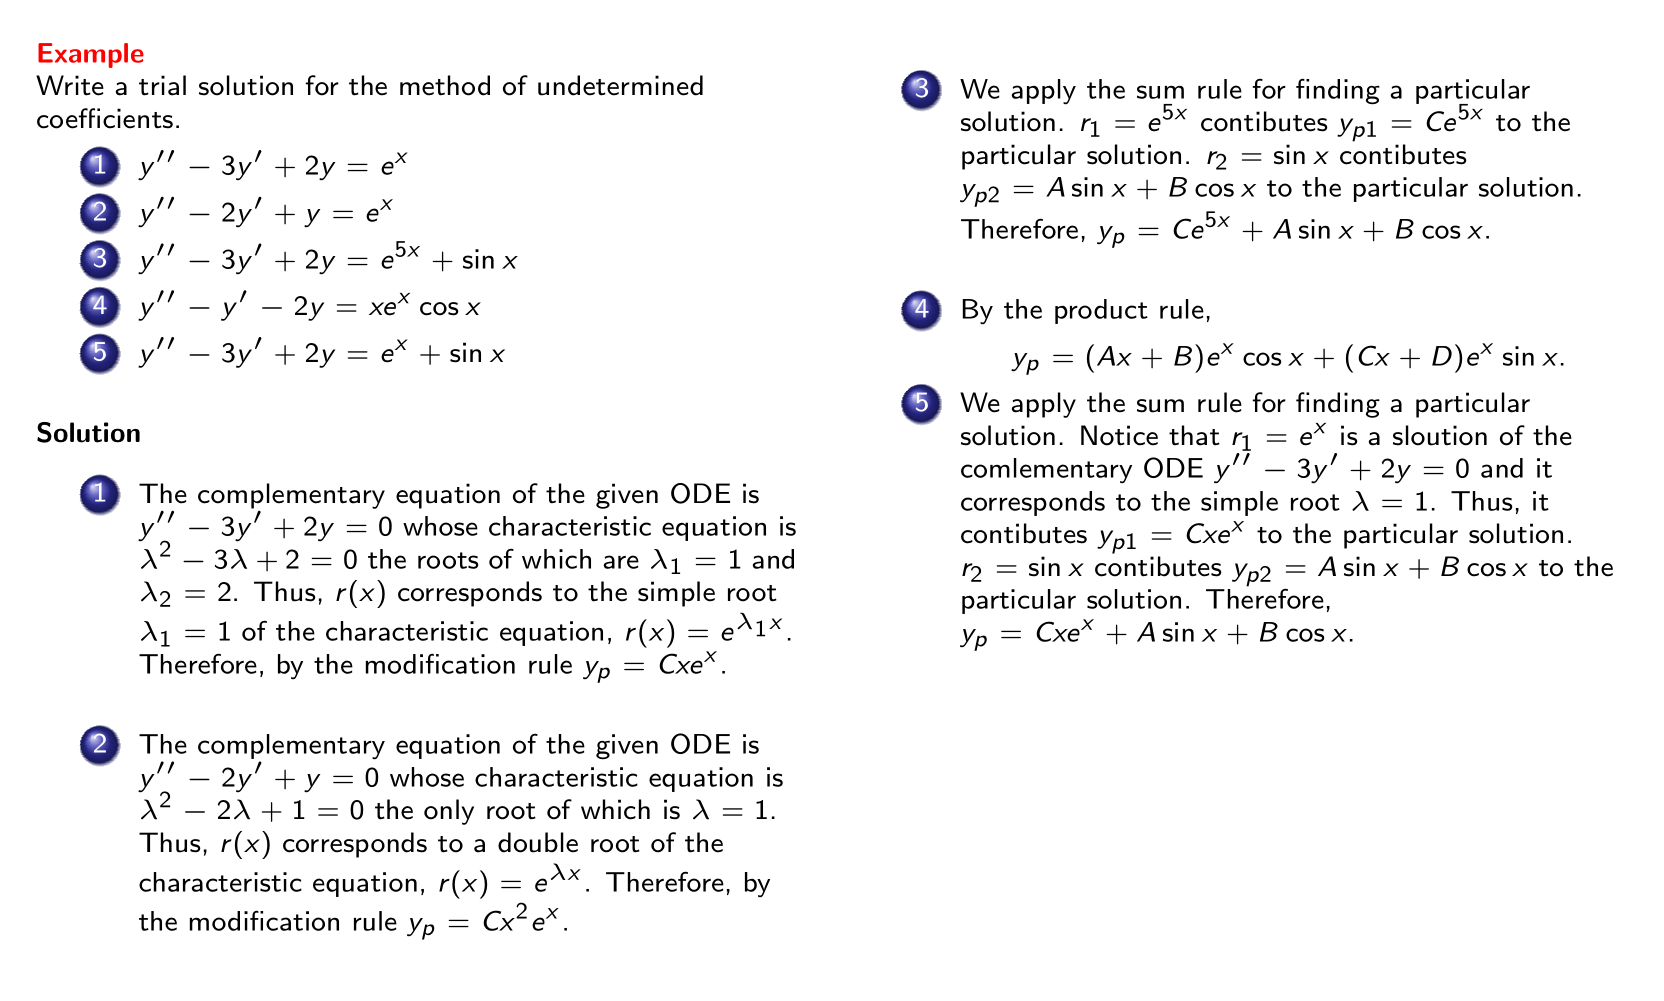
\includegraphics[scale =0.4]{images/exs.png}
    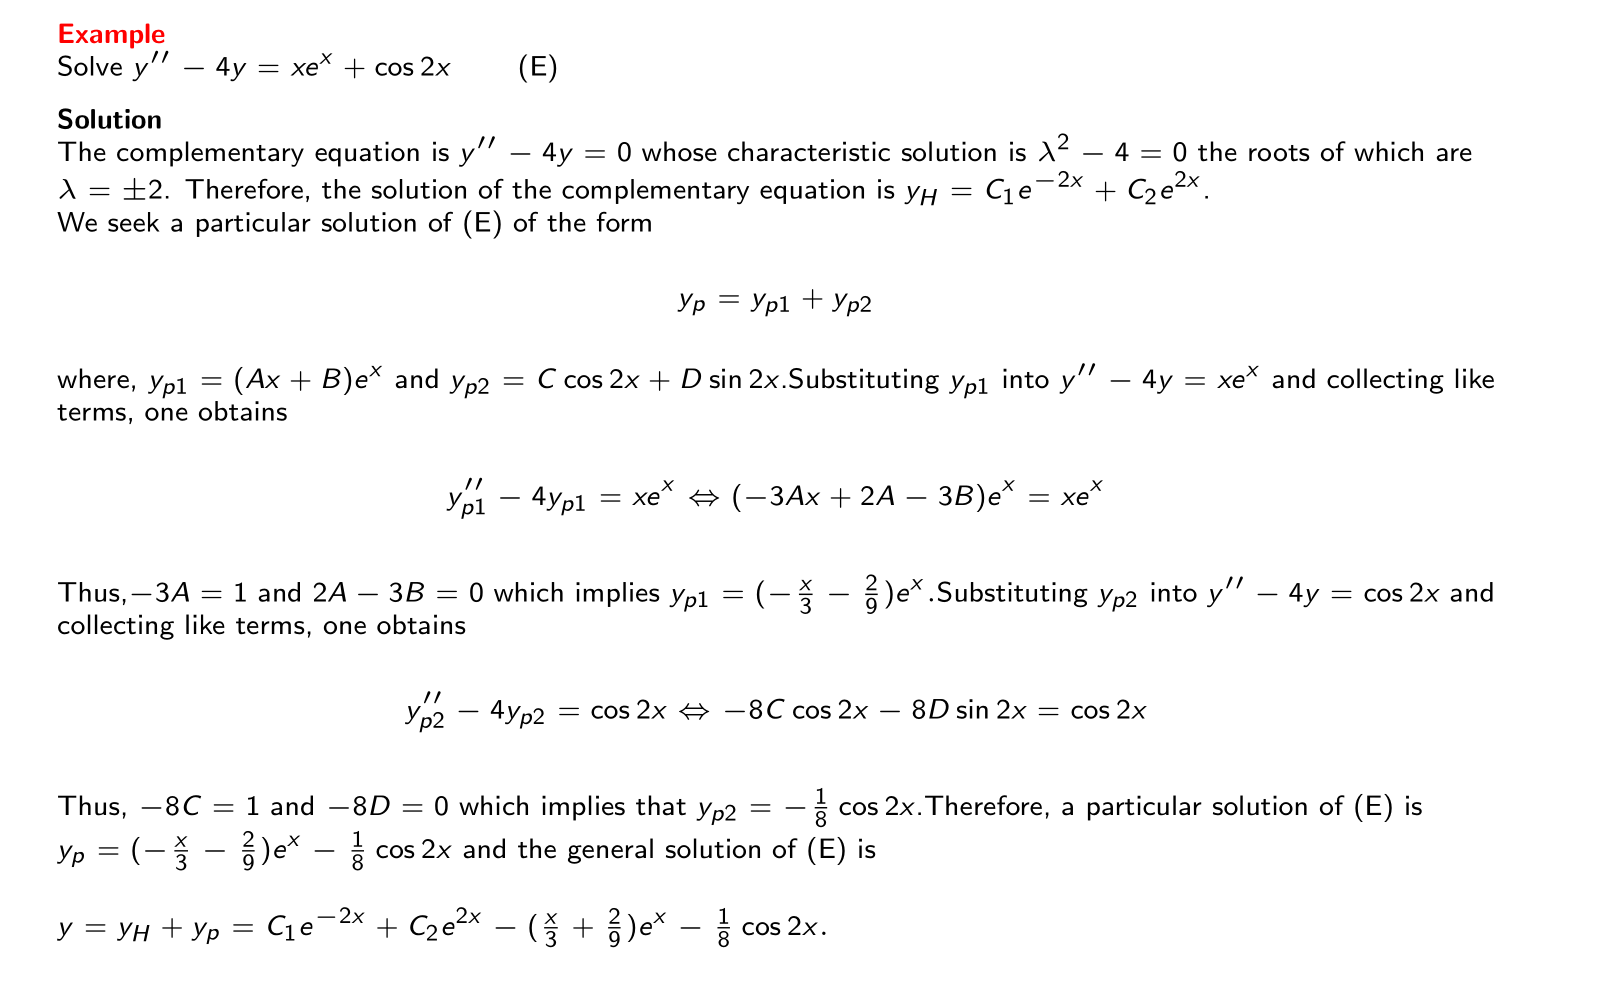
\includegraphics[scale =0.4]{images/ex.png}
\end{center}
\subsection{Method of variation of parameters}
this is the general method used to solve NH ODEs.\\
in very simple terms 
\begin{enumerate}
    \item find $y_1, y_2$ from $y_H$
    \item find $u_1,u_2$ as follows :
    \begin{align*}
        u_1 &= -\int \frac{r(x) y_2}{W} dx & u_2 &= \int \frac{r(x) y_1}{W} dx&
        W &= \begin{vmatrix}
        y_1&y_2\\
        y_1'&y_2'\\
            \end{vmatrix}
           & \text{W is called the Wronskian}
    \end{align*}
\end{enumerate}
\subsection{Where did this information come from ?}
after finding $y_1 \text{and} y_2$ we suppose that $y_p = u_1(x)y_1 + u_2(x)y_2$\\
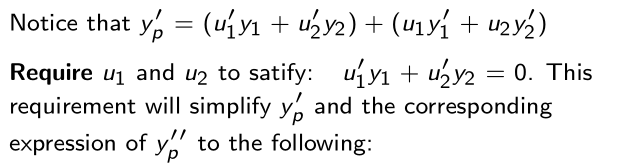
\includegraphics[scale= 0.6]{images/111.png}\\
\begin{center}
    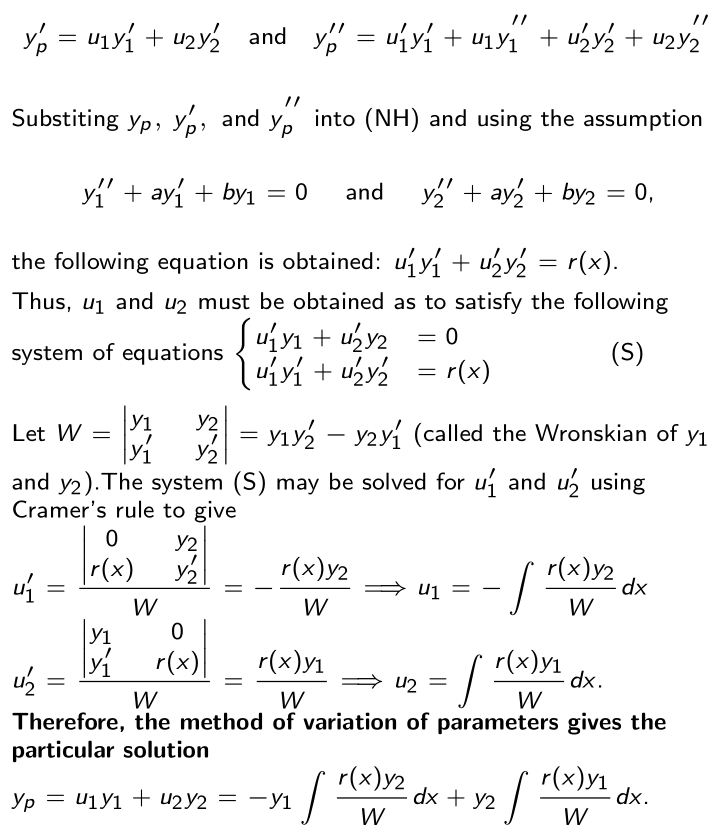
\includegraphics[scale= 0.5]{images/222.png}
\end{center}
\subsection{Vibrating Springs}
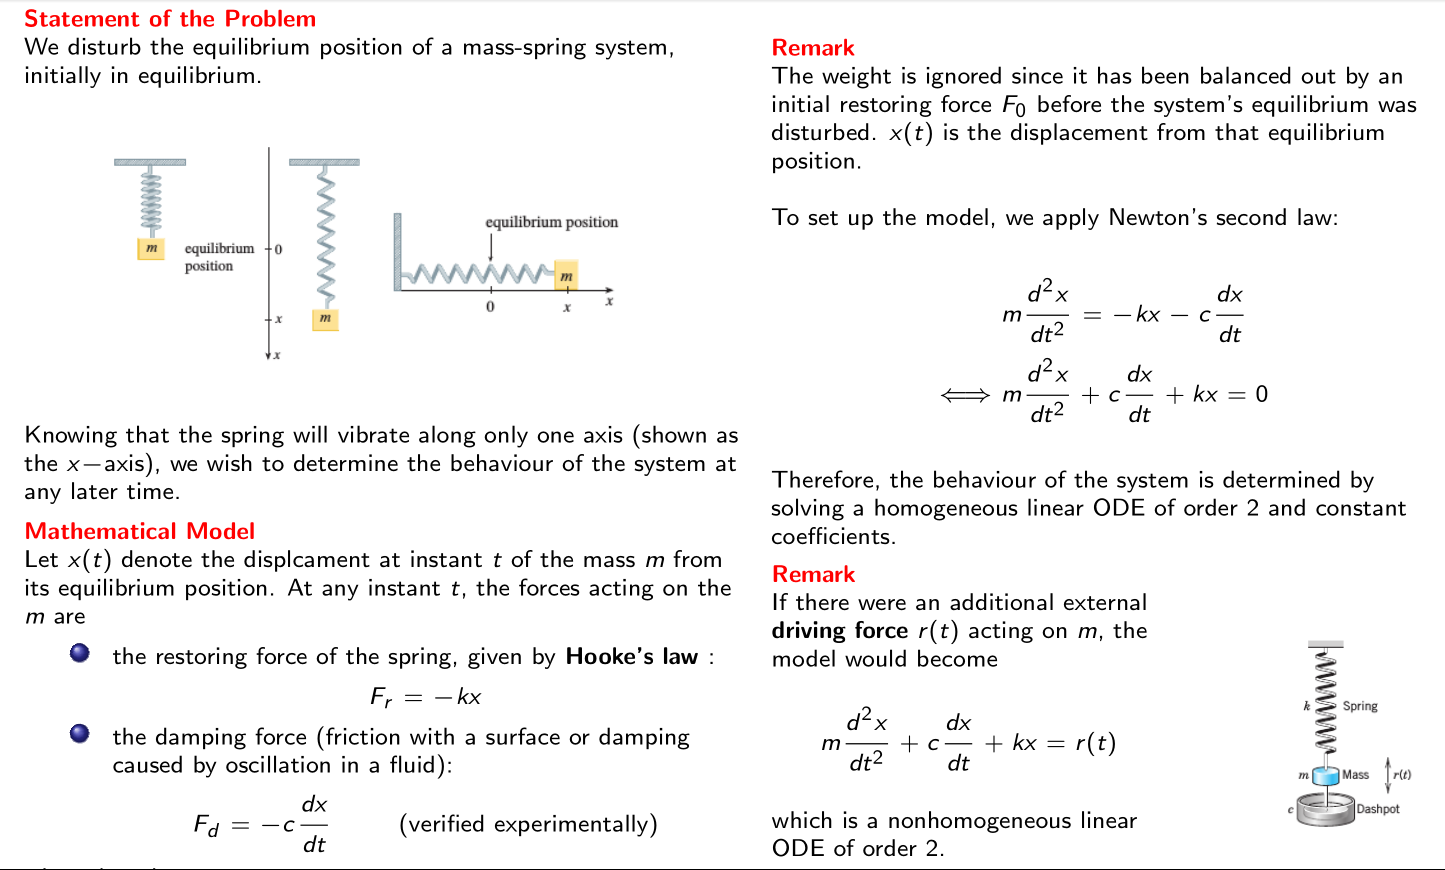
\includegraphics[scale = 0.45]{images/vb1.png}\\
\line(1,0){250}\\
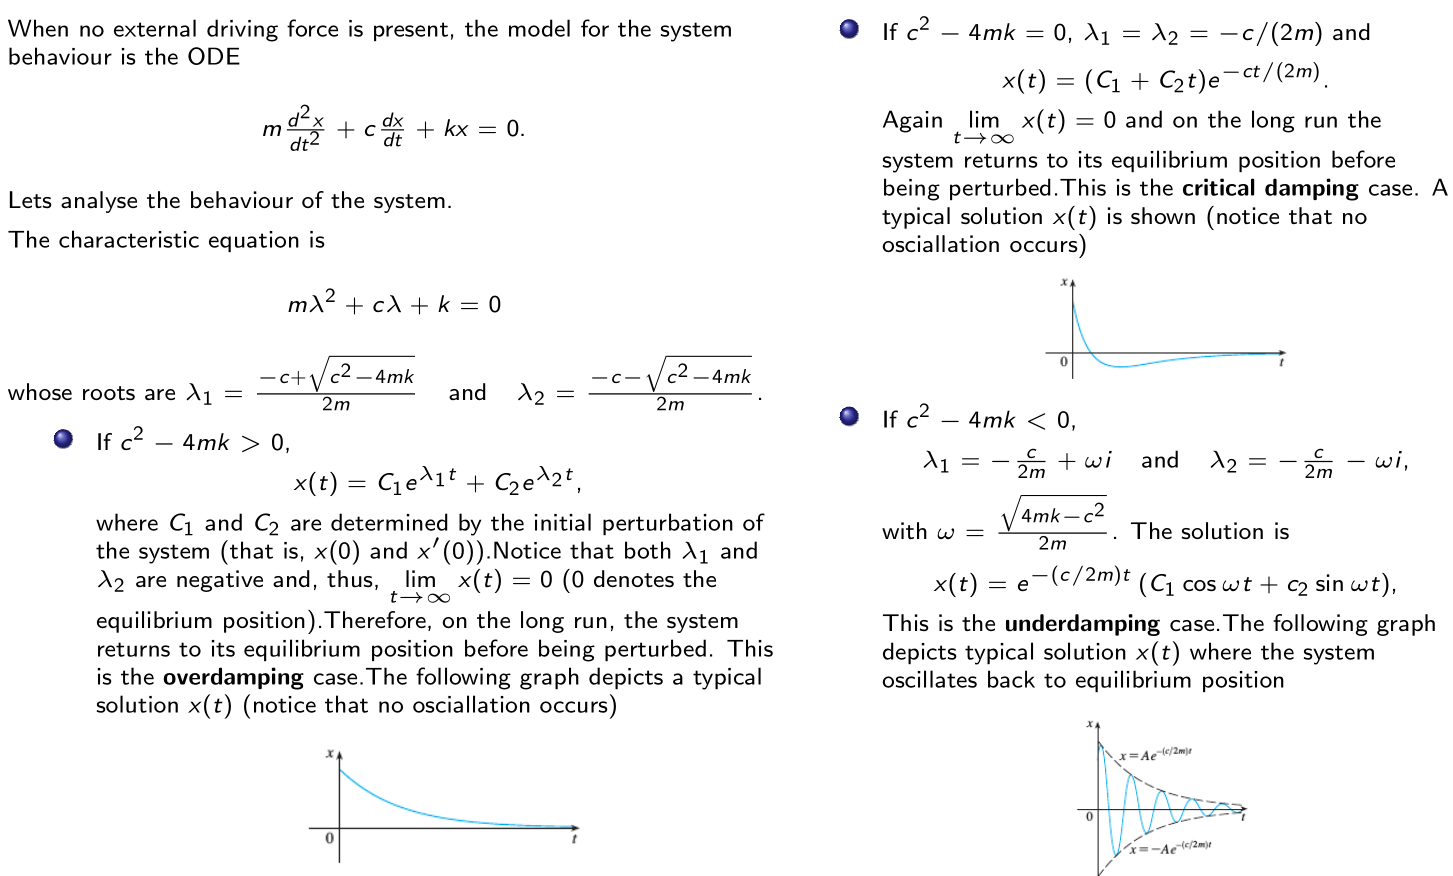
\includegraphics[scale = 0.45]{images/vb2.png}\\
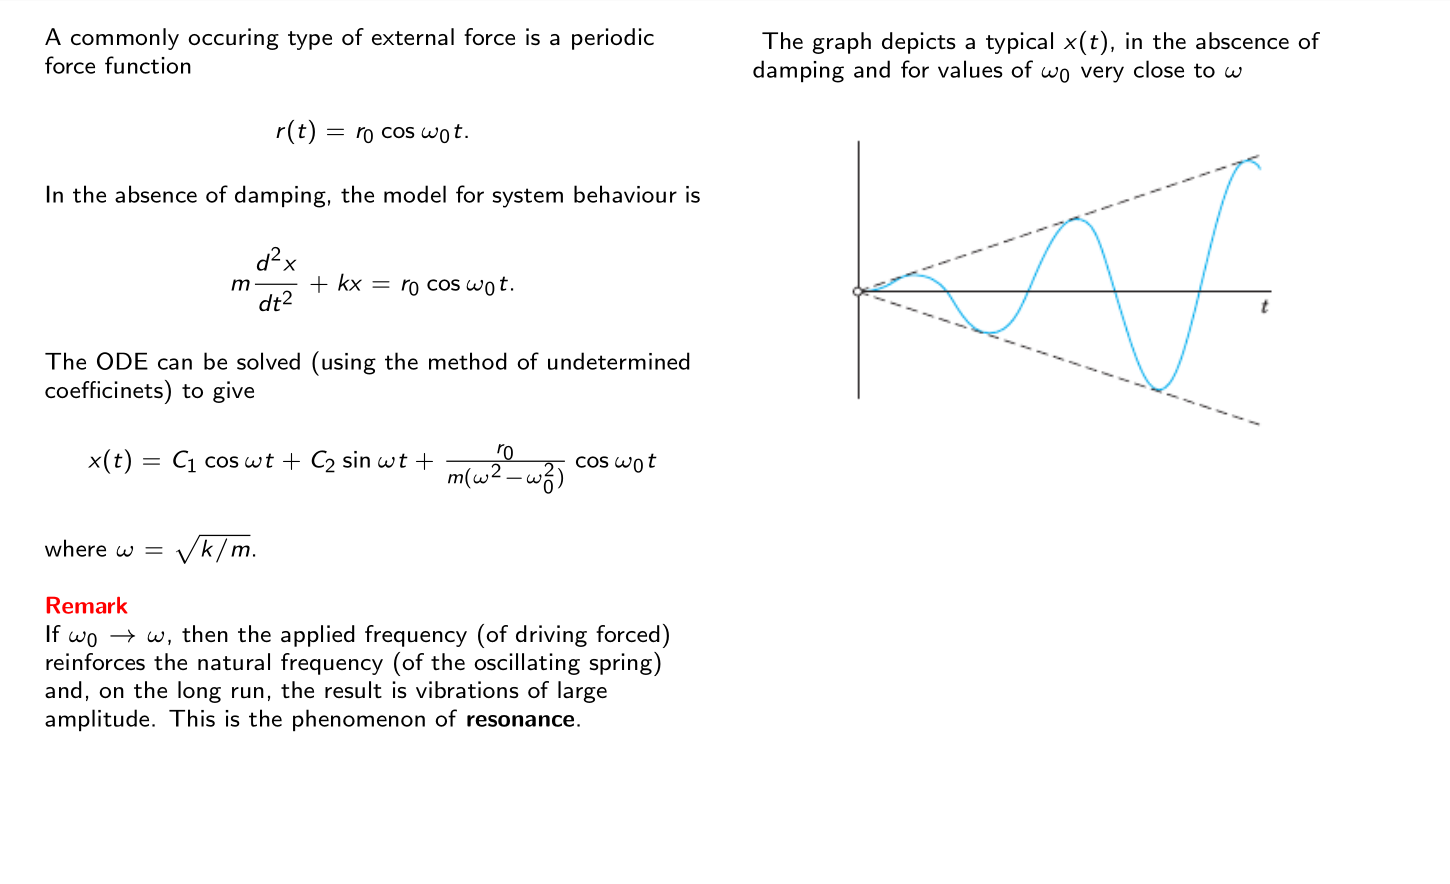
\includegraphics[scale = 0.48]{images/vb3.png}
\section{Worksheet Notes}
\subsection{Worksheet 8}

\end{document}
